%!TEX program = xelatex
\documentclass[cn,hazy,pku,12pt,normal,math=newtx,cite=super]{elegantnote}
\title{燃烧热的测定}

\author{刘松瑞 \quad 2100011819 \\ 组号:24 \quad 组内编号:5}
\institute{化学与分子工程学院}

\expdate{\zhdate{2023/11/30}}
\temperature{16.3 \si{^{\circ}C}}
\pressure{102.26 \si{kPa}}

\usepackage{gensymb}
\usepackage{array}
\usepackage{subfigure}
\usepackage[fontset=windows]{ctex}
\usepackage{graphicx}
\usepackage{float}
\usepackage{caption}
\usepackage{multirow}
%\usepackage{subfig}
%\usepackage{float}
\begin{document}

\maketitle

\abstracts{
    本实验有三轮实验,分别测定蔗糖、苯甲酸以及奶片的燃烧热
    。通过已知的苯甲酸燃烧热测定了氧弹的水当量,使用雷诺校正法修正了
    燃烧过程中环境热交换,最后测定奶片的恒容燃烧热。
    
    实验得到,得到每克蔗糖温升值为 $\Delta T_m = 0.098\ K/g$ ,
    量热计常数为 $ W = 2553 \pm 9 J/K$,奶片的燃烧热 $Q_V = 1.972 \times 10^4 \pm 2 \times 10^1\ J/g$
    ,实验中误差的主要来源是容量瓶的定容误差。
}
\keywords{氧弹式量热计\quad 燃烧热\quad 雷诺校正
}

\newpage


\section{引言}

\subsection{实验目的、原理与方法}

实验目的、原理与方法详见预习报告图~\ref{1}。 \cite{pcl2002}

\begin{figure}[htbp]
    \centering
    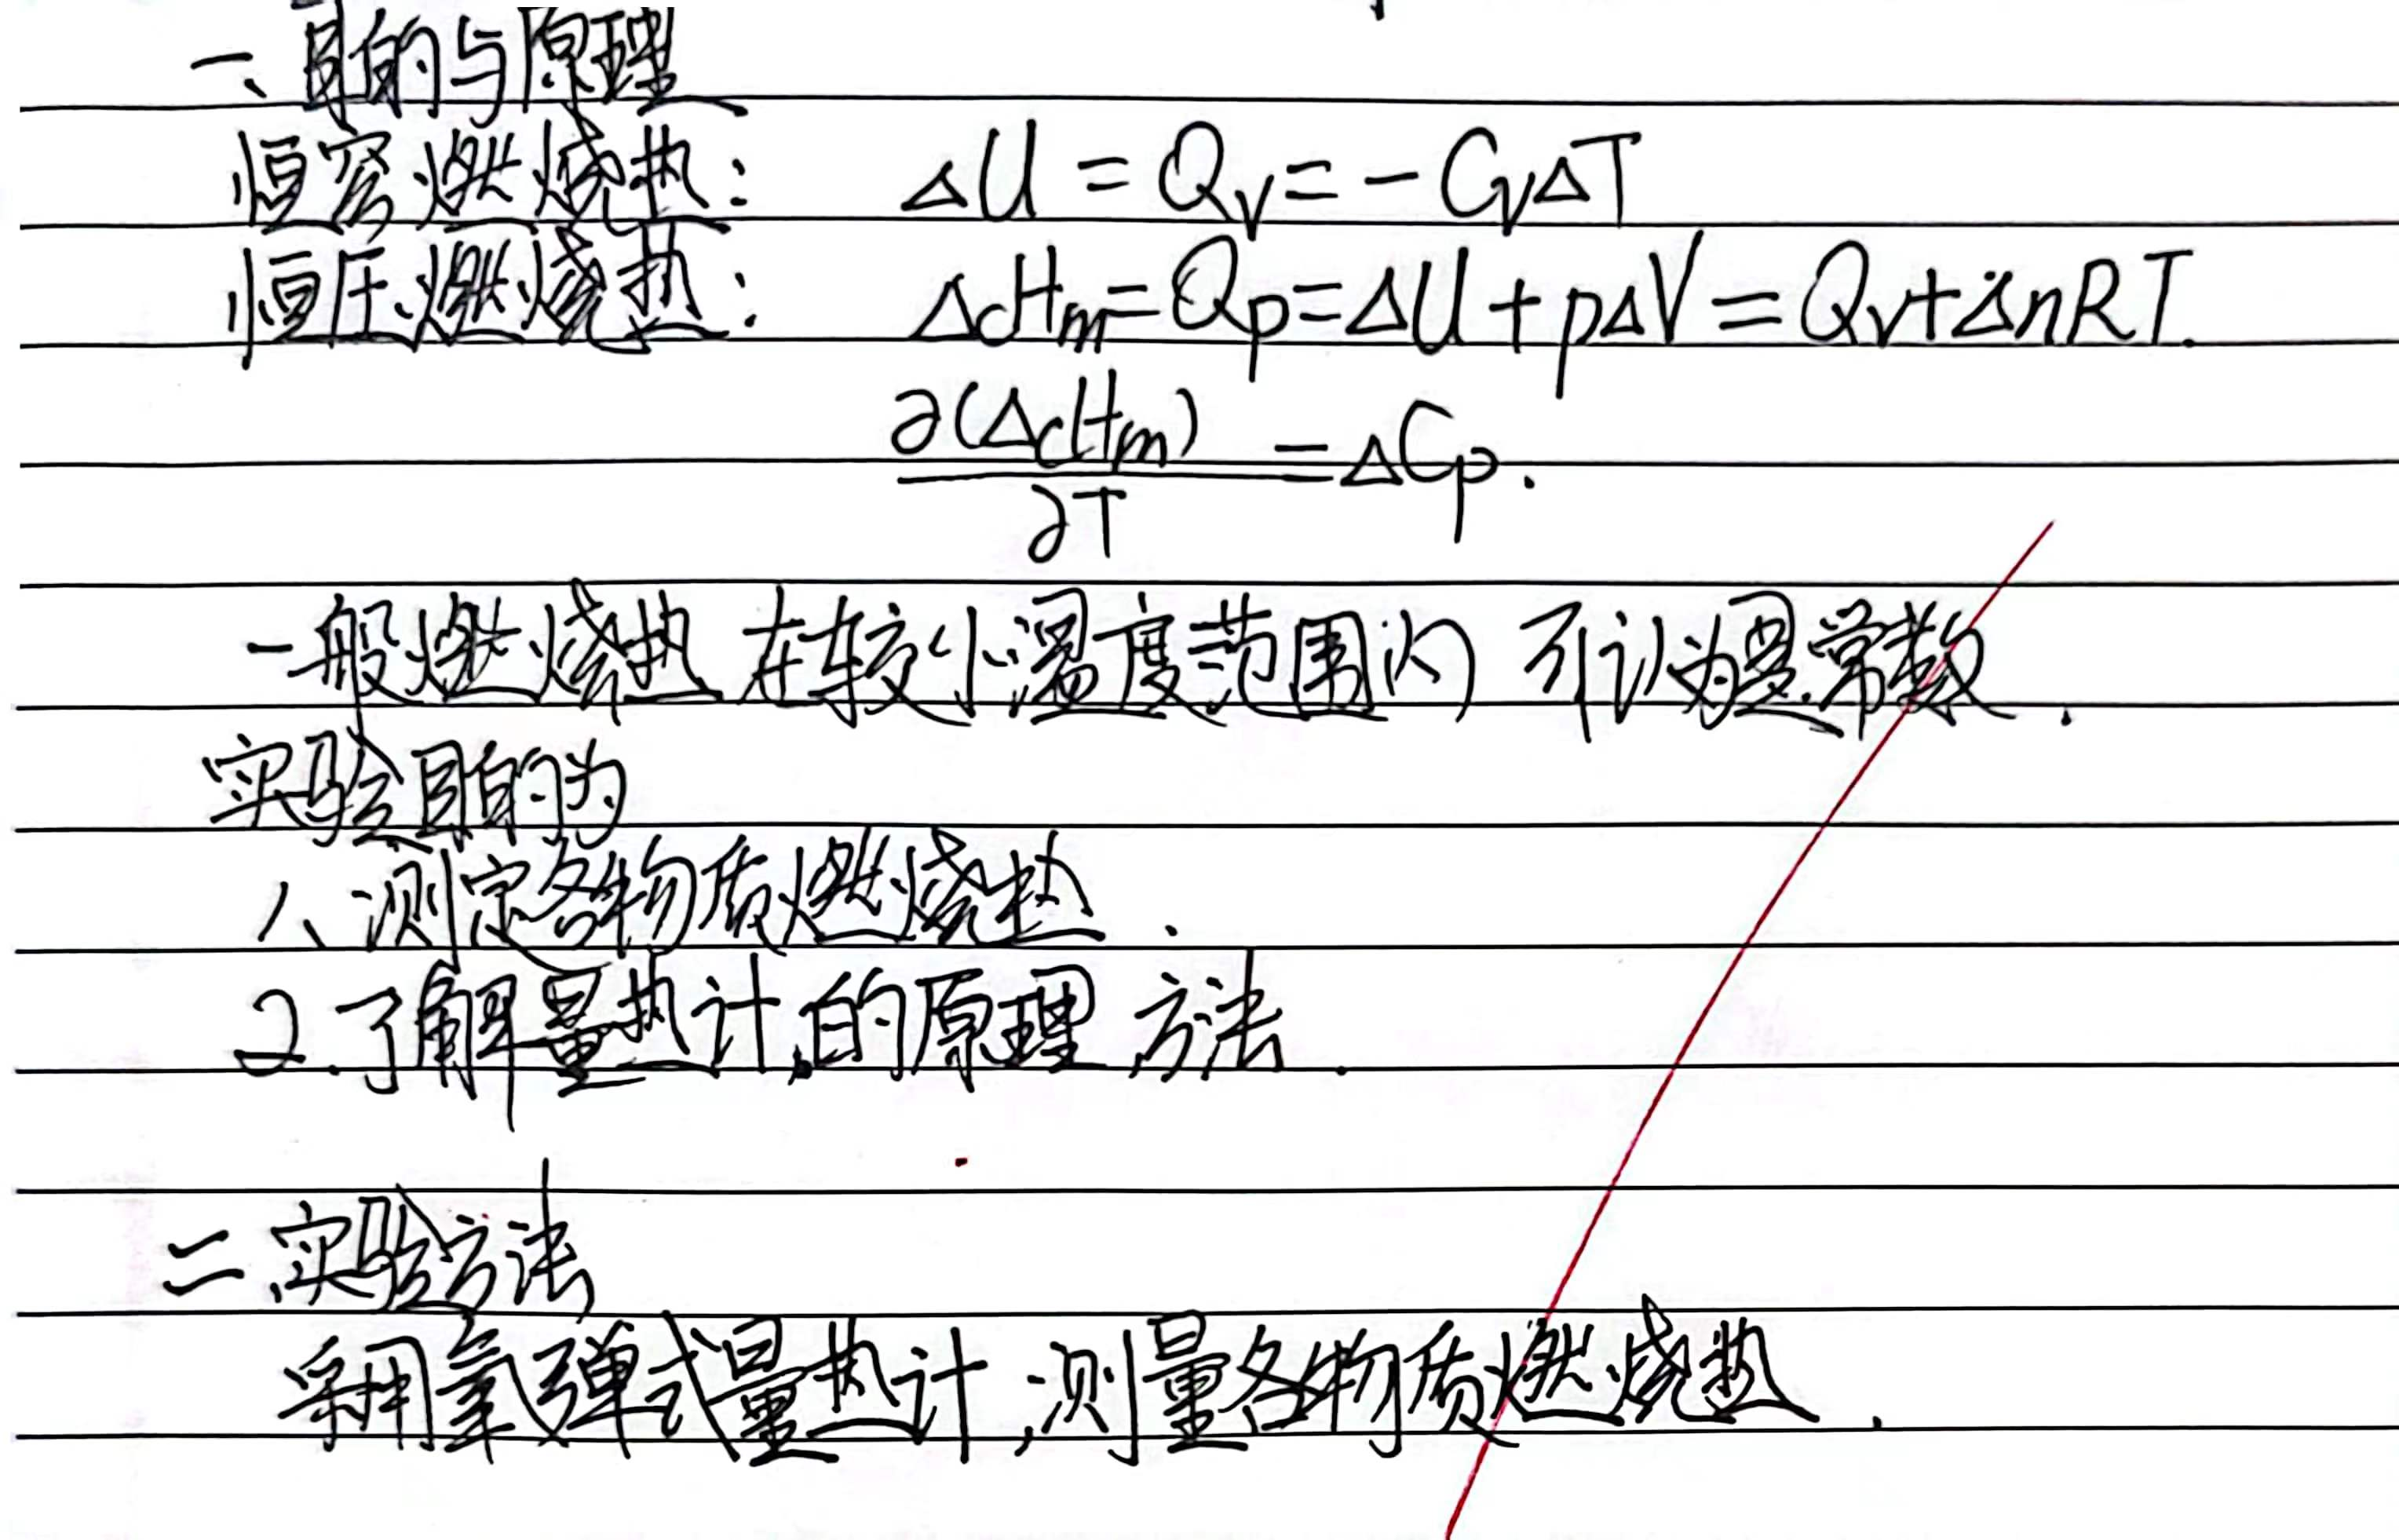
\includegraphics[width = .70\textwidth]{image/yxbg_1.jpg}
    \caption{实验的目的与原理}\label{1}
\end{figure}

\section{实验部分}

\subsection{实验步骤}
实验步骤详见预习报告图~\ref{2} 和 \ref{3}。

\begin{figure}[htbp]
    \centering
    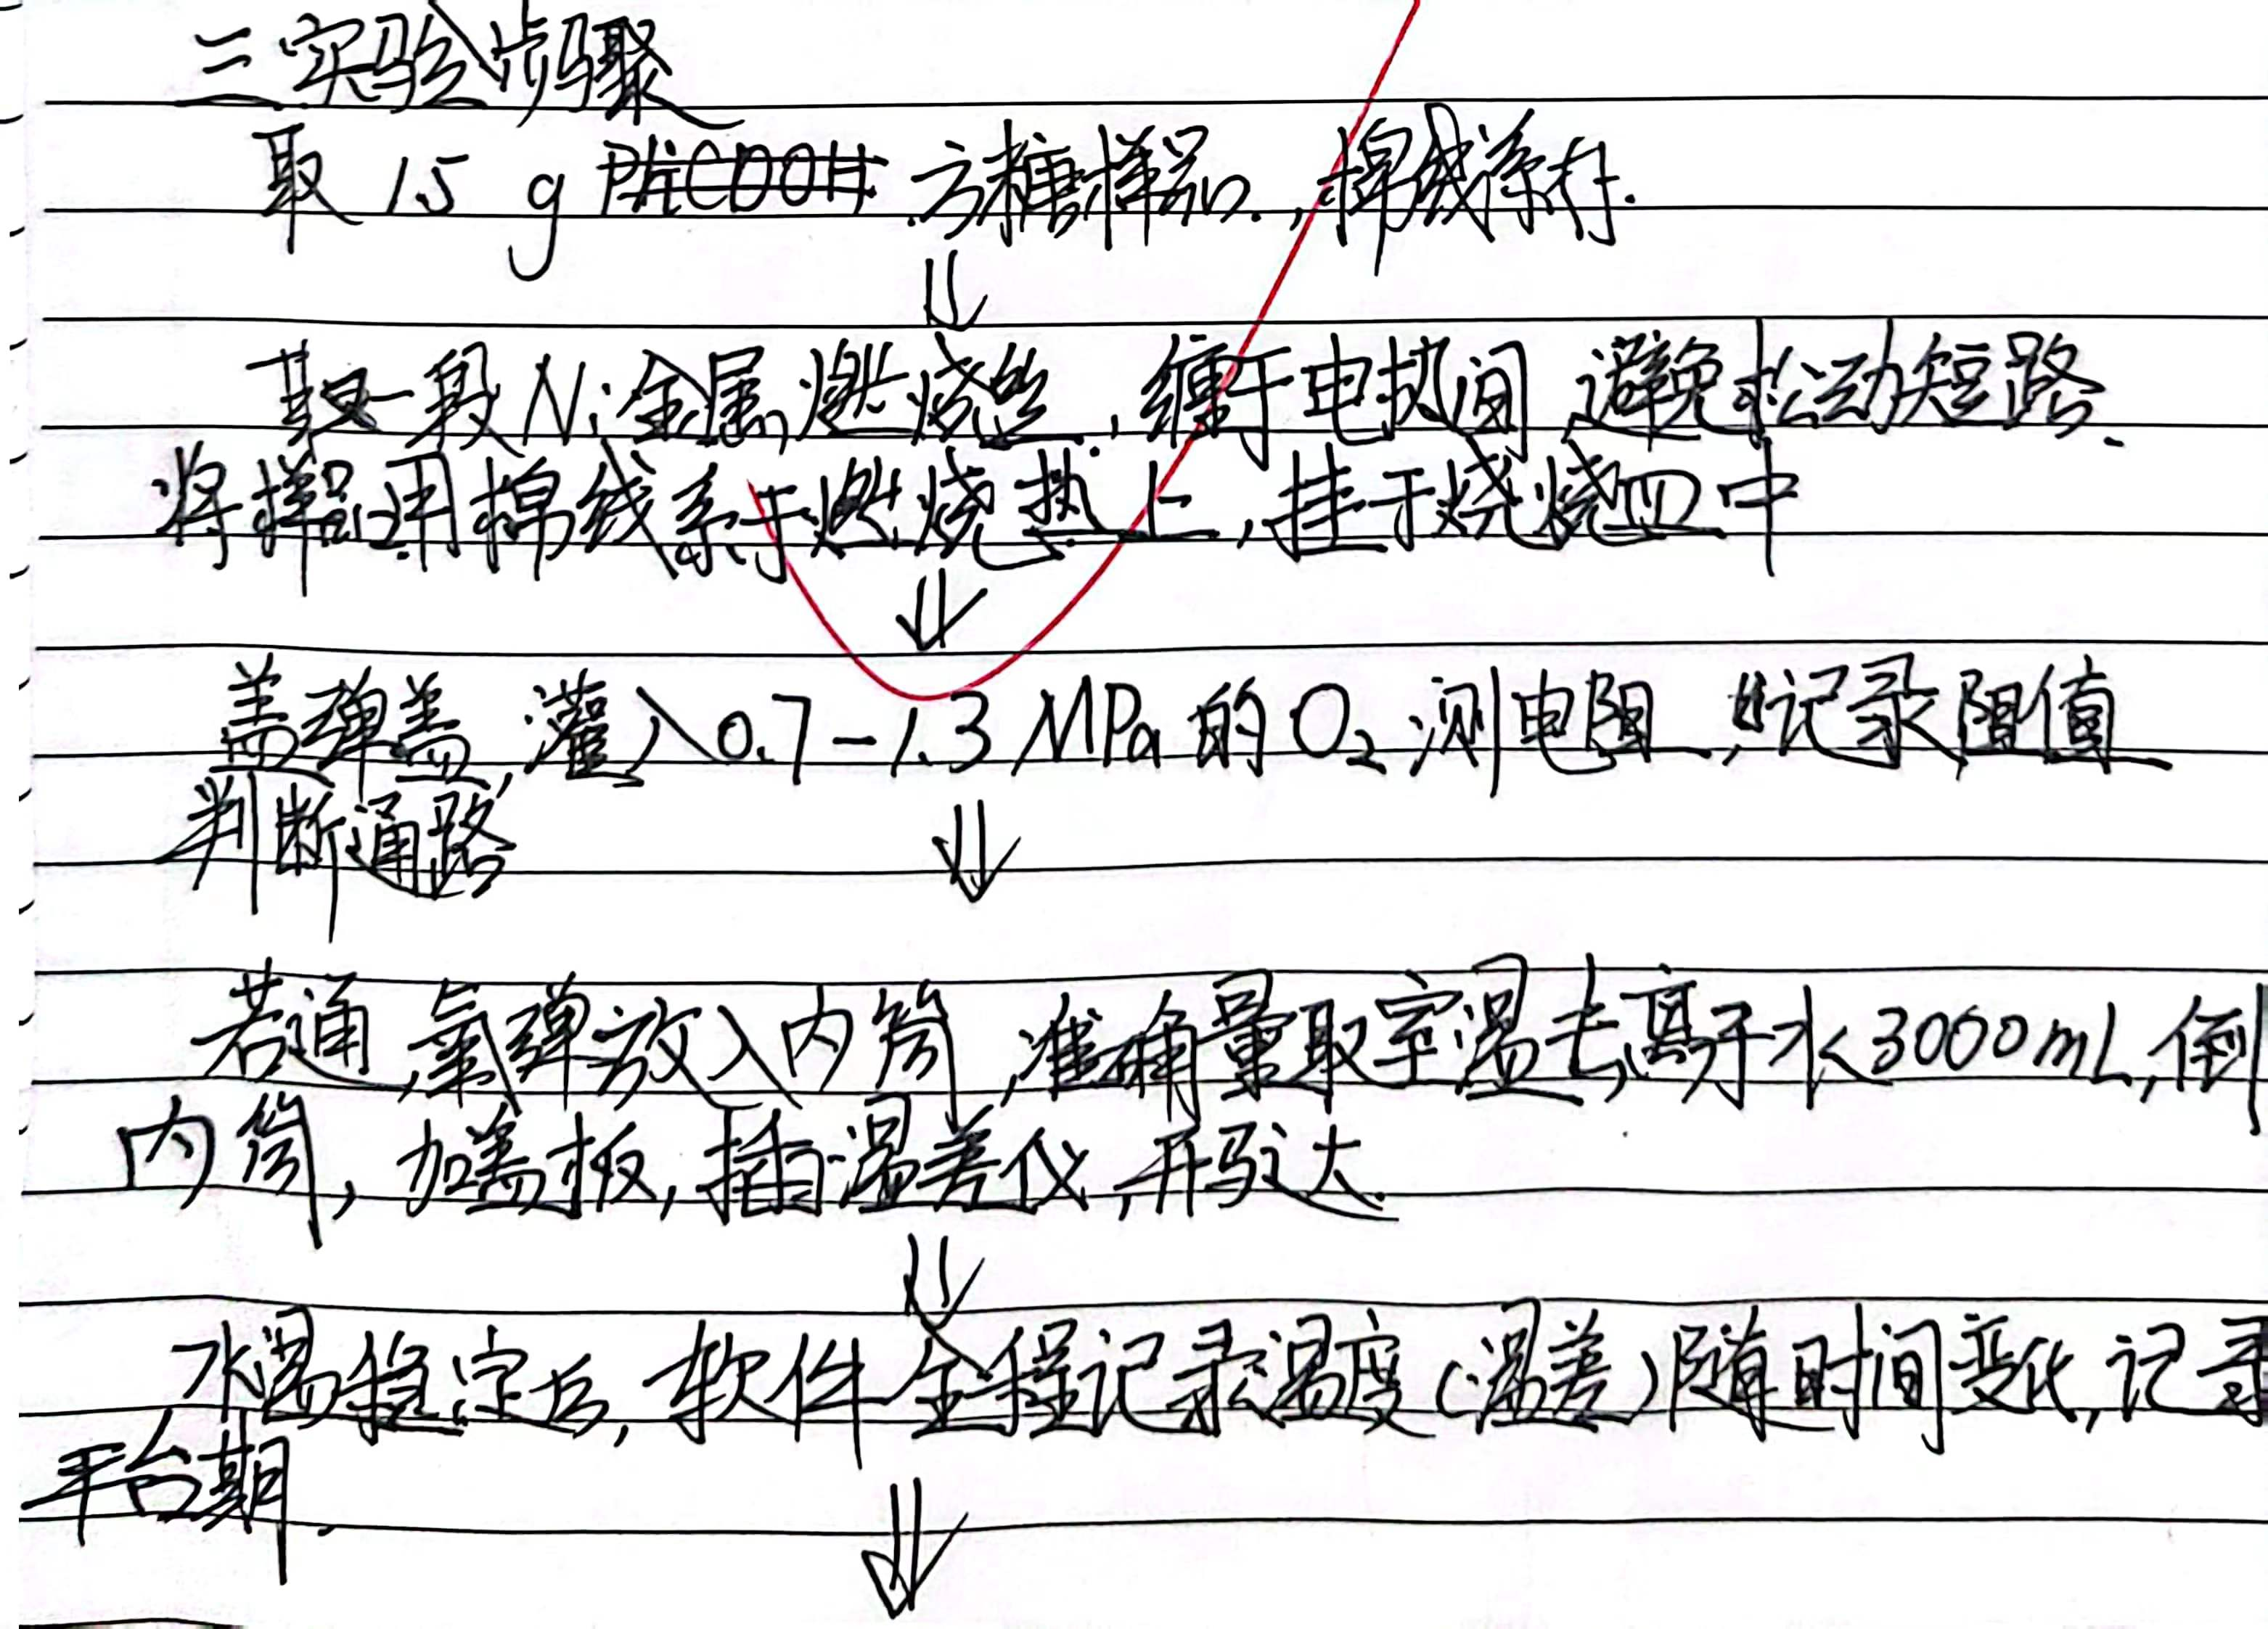
\includegraphics[width = .70\textwidth]{image/yxbg_2.jpg}
    \caption{实验的目的与原理}\label{2}
\end{figure}

\begin{figure}[htbp]
    \centering
    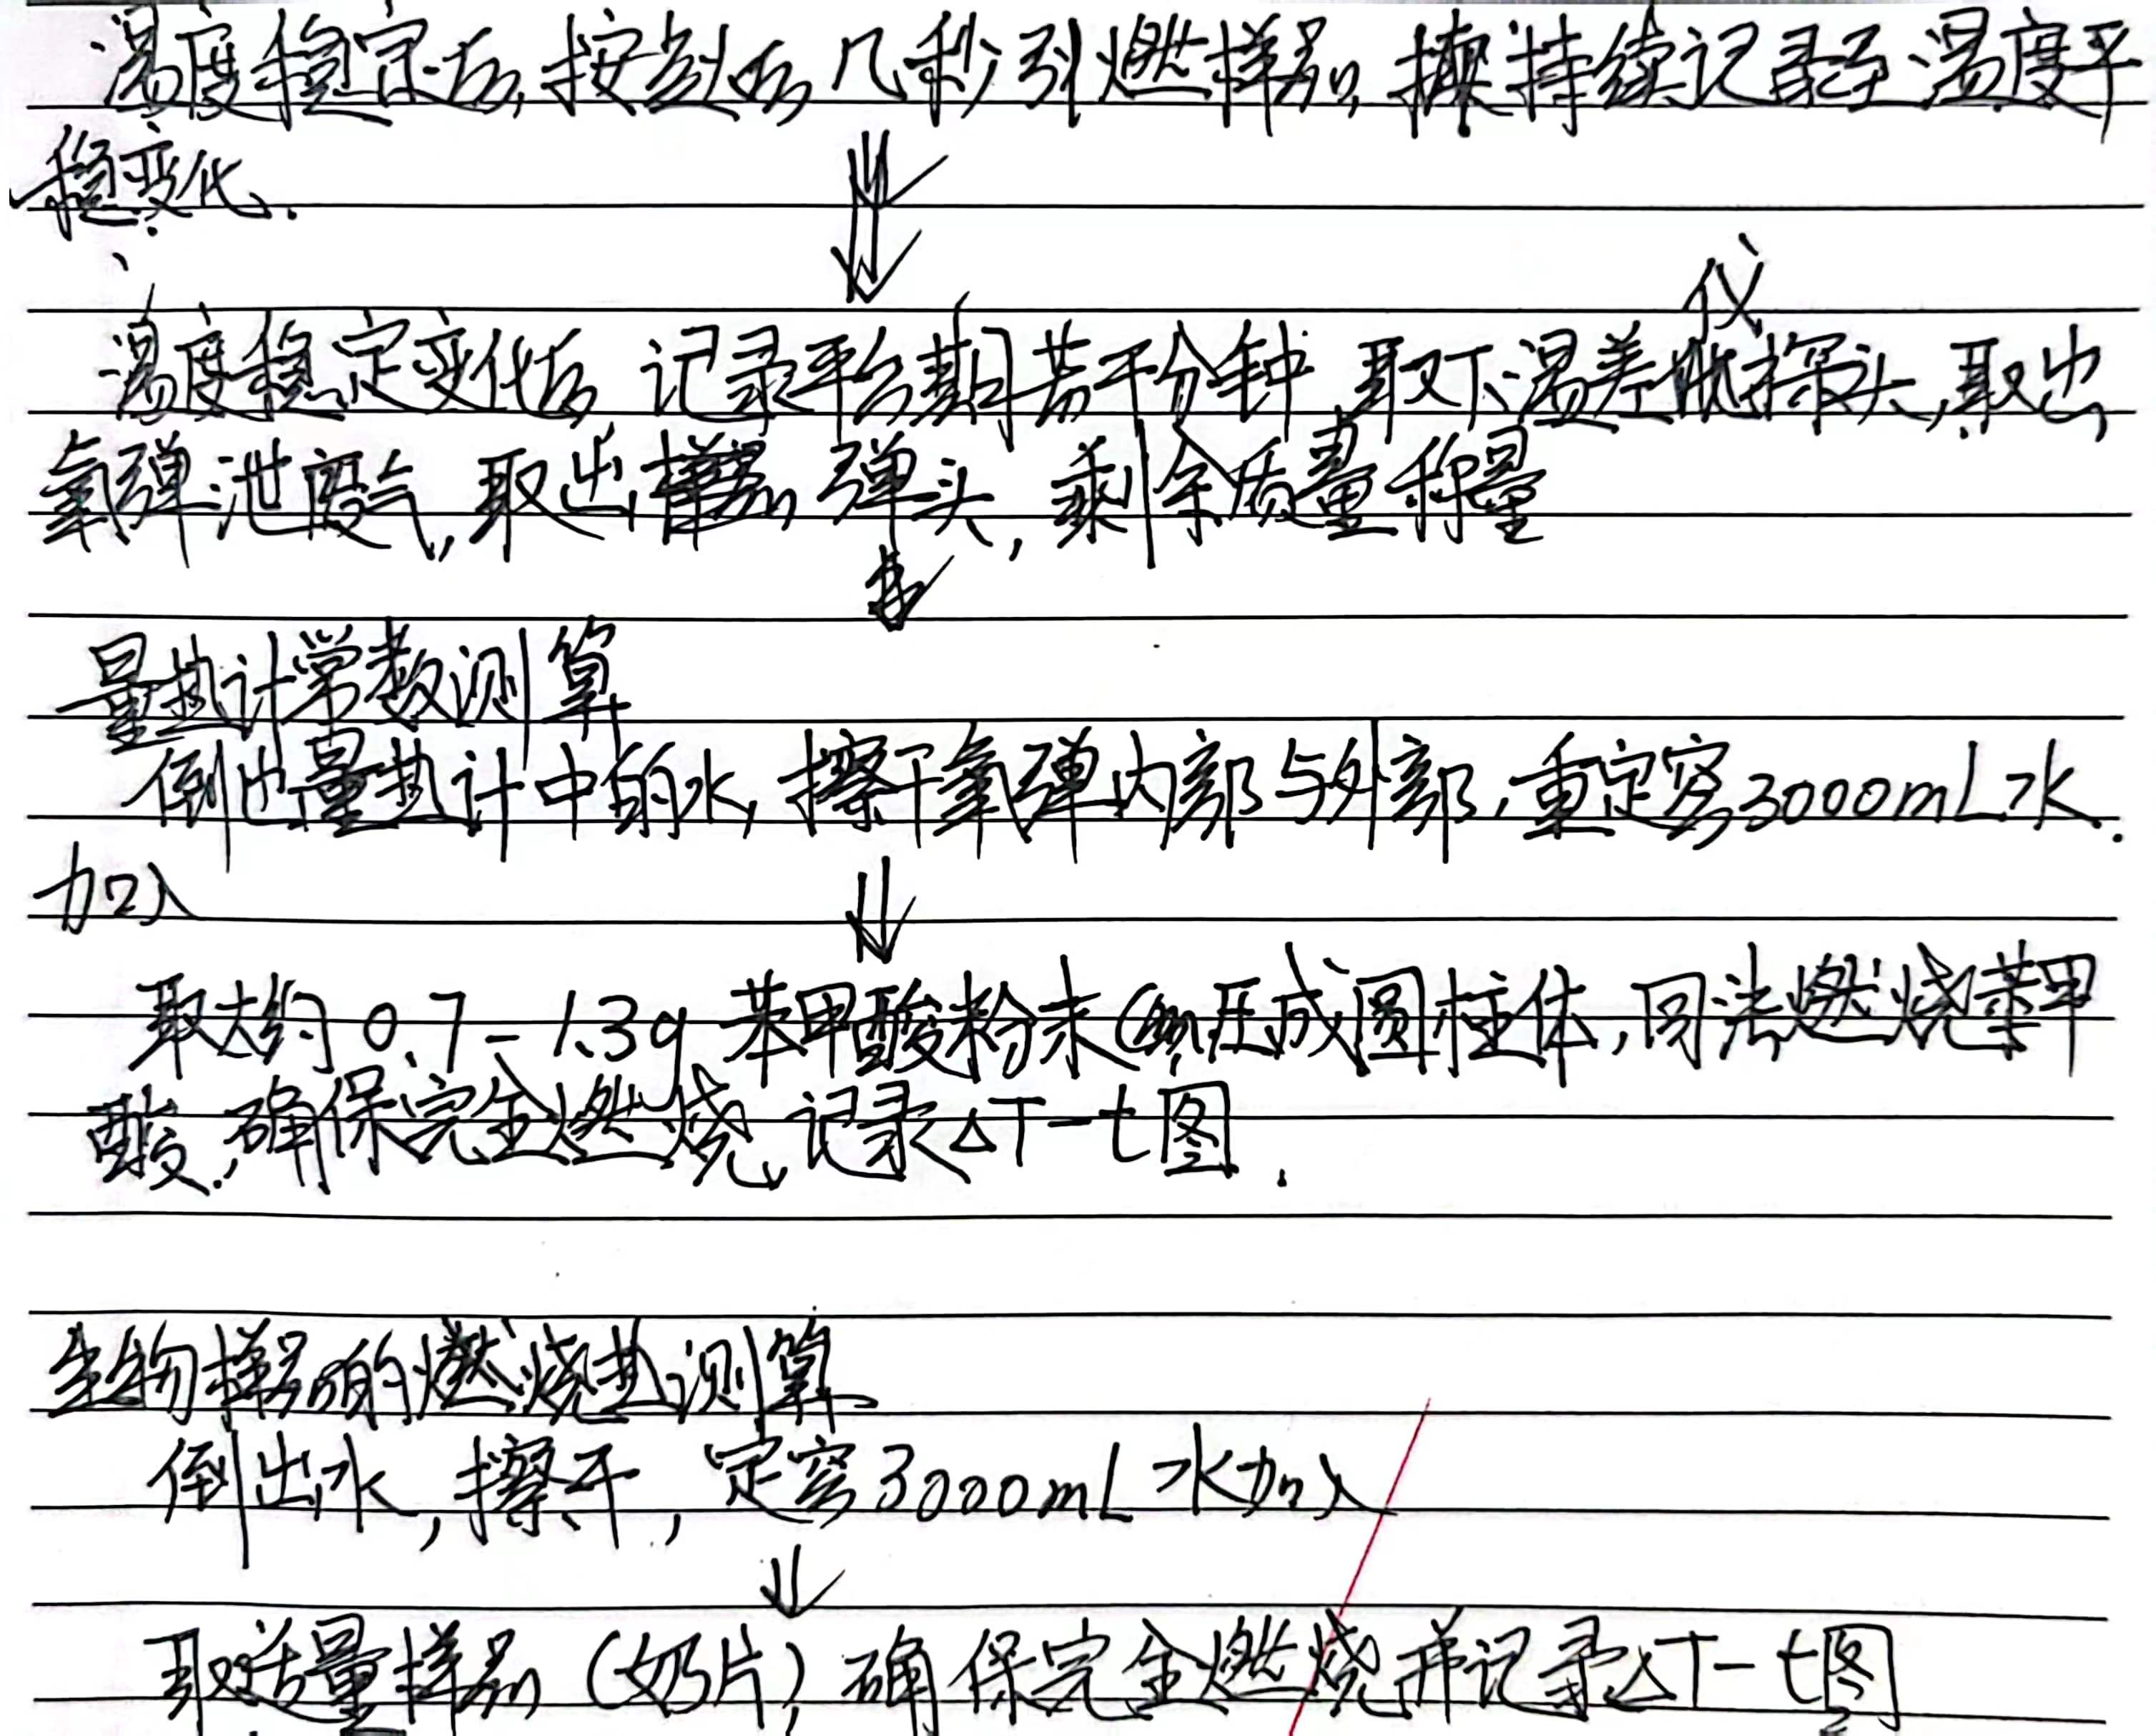
\includegraphics[width = .70\textwidth]{image/yxbg_3.jpg}
    \caption{实验的目的与原理}\label{3}
\end{figure}

\subsection{仪器与药品}

\begin{enumerate} %有序列表
    \item 试剂 \\   镍丝,棉线,苯甲酸,蔗糖,奶片;
    \item 仪器 \\   氧弹式量热计,氧气钢瓶,压片机,温差测量仪,容量瓶,万用表。
\end{enumerate}

\section{实验现象与数据处理}
\subsection[short]{第一轮实验}
使用氧弹式量热计测量蔗糖的燃烧热,称量蔗糖 1.5037 g ,测得固定的棉线 0.0179 g ,燃烧丝镍丝 0.0183 g。
点燃,测得燃烧的温差随时间变化图如图 \ref{4} 所示。

\begin{figure}[htbp]
    \centering
    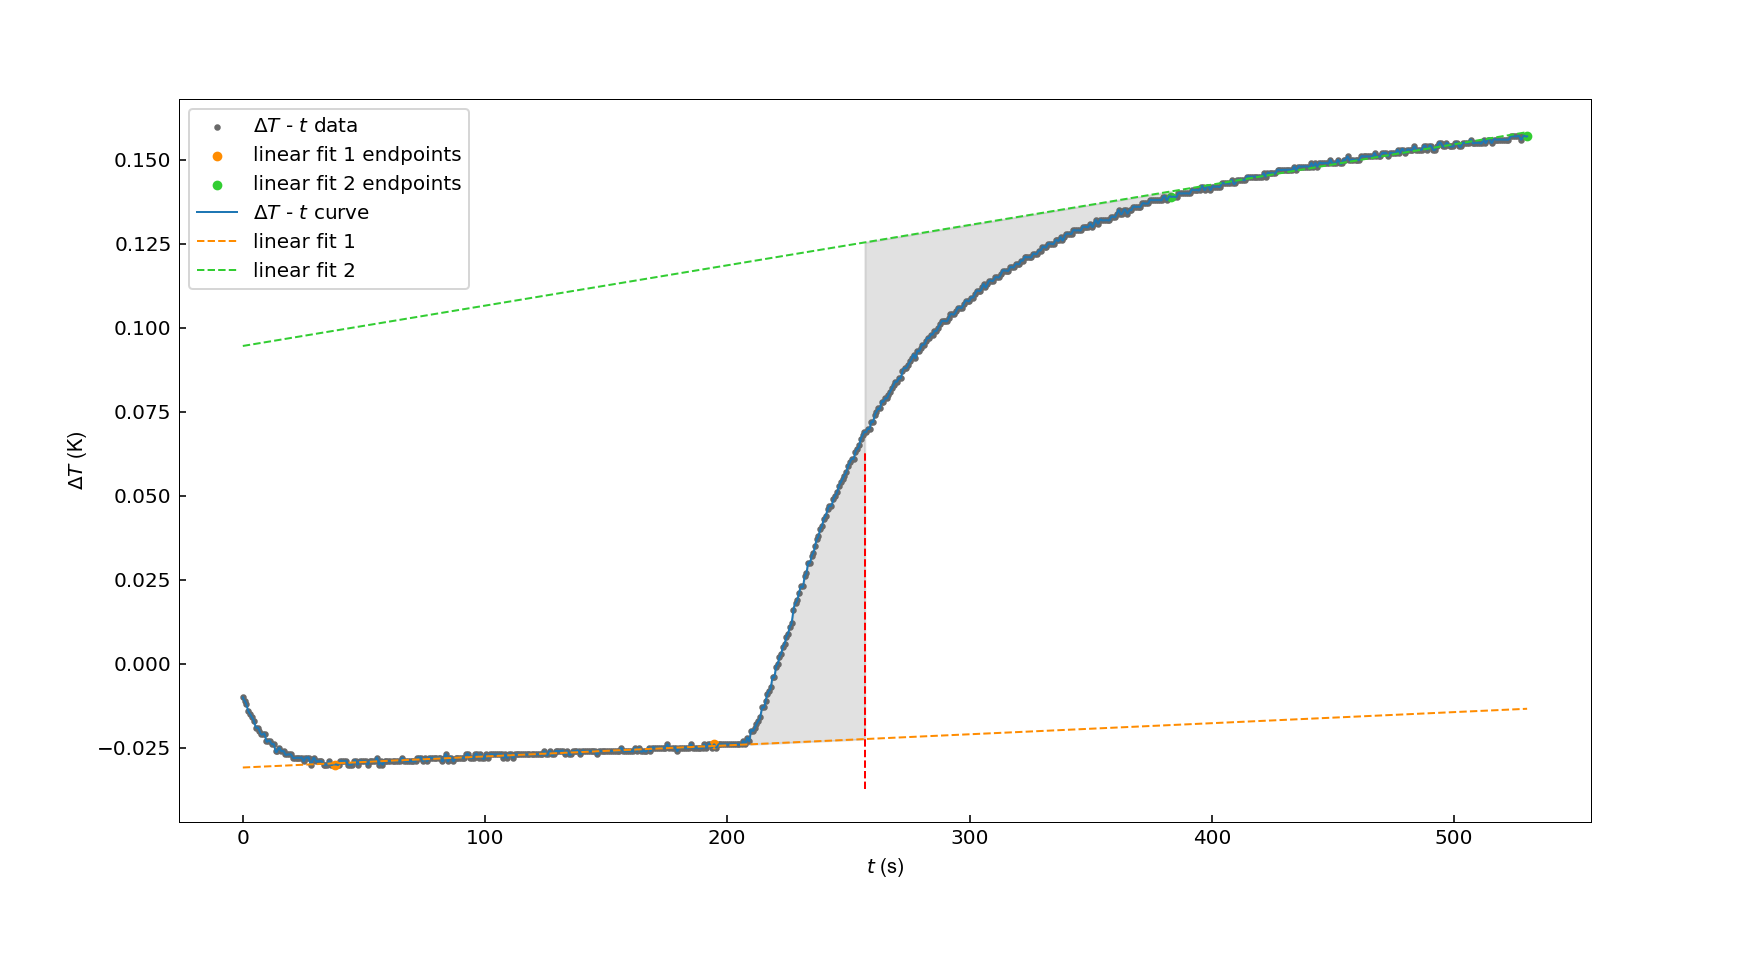
\includegraphics[width = .90\textwidth]{image/r1.png}
    \caption{第一轮实验温差随时间变化图}\label{4}
\end{figure}

使用雷诺校正可以得到燃烧前后的温度 $T_{before} = -0.022\ K\ T_{after} = 0.125\ K$ ,温差为 $\Delta T = 0.147\ K$。
得到每克样品温升值为:
$$
\Delta T_m = 0.098\ K/g
$$

\begin{figure}[htbp]
    \centering
    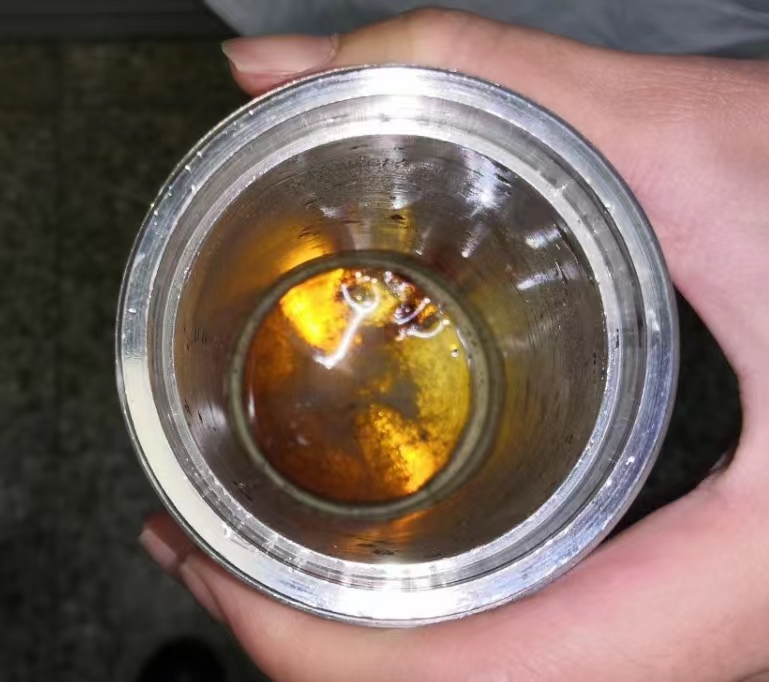
\includegraphics[width = .70\textwidth]{image/cwtp.jpg}
    \caption{第一轮实验燃烧产物图片}\label{5}
\end{figure}

本次燃烧得到的升温量相比于同组成员显著小,得到的燃烧后物质为深黄色液体如图 \ref{5} ,粘度较高,有淡香味。疑似由于燃烧不充分得到了焦糖液体。
可能导致出现这样的原因为:

1. 氧弹式量热计漏气,没有充分充入氧气,但是在加热前已经灌入 1 MPa 的氧气,若存在严重漏气应当在浸入水中有气泡产生,因此可能性较小

2. 氧弹式量热计漏水,但是充入氧气后体系呈负压,很难有水进入。

3. 在加热时,按下加热键时间过短,燃烧丝加热时间较短。可能反应过程为:燃烧丝引燃了棉线,但是没有引燃蔗糖,蔗糖掉落,棉线的燃烧加热体系温度,使蔗糖变成焦糖。

综上,笔者倾向于第三种原因。在后面的实验均延长了加热时间,使样品充分燃烧。

\subsection[short]{第二轮实验}\label{114}

使用氧弹式量热计测量苯甲酸的燃烧热,称量苯甲酸 0.8849 g ,测得固定的棉线 0.0226 g ,燃烧丝镍丝 0.0141 g。
点燃,测得燃烧后的镍丝质量为 0.0069 g ,温差随时间变化图如图 \ref{6} 所示。

\begin{figure}[htbp]
    \centering
    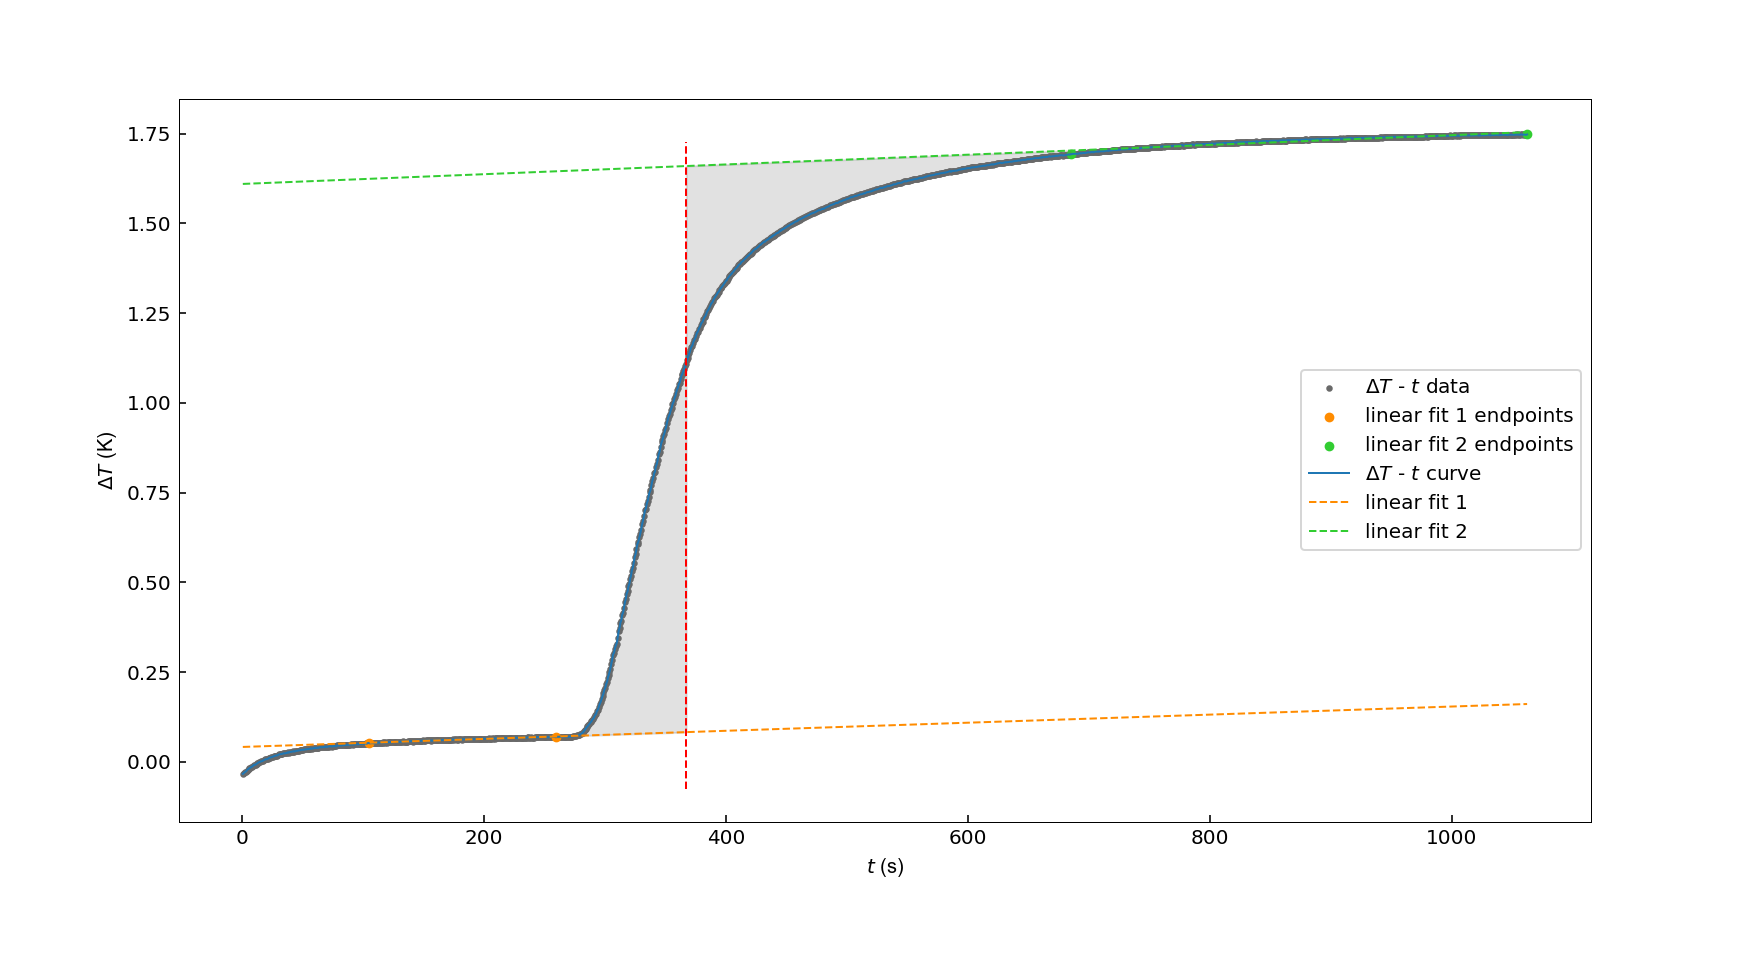
\includegraphics[width = .90\textwidth]{image/r2.png}
    \caption{第二轮实验温差随时间变化图}\label{6}
\end{figure}


使用雷诺校正可以得到燃烧前后的温度 $T_{before} = 0.083\ K,\ T_{after} = 1.660\ K$ ,温差为 $\Delta T = 1.577\ K$。
得到每克样品温升值为:
$$
\Delta T_m = 1.782\ K/g
$$

由公式
$$
(W+DC_{H_2O})\Delta T = -Q_VG-\sum{q}
$$

可得
$$
W = \frac{-Q_VG-\sum{q}}{\Delta T}-DC_{H_2O}
$$

由此公式可以计算量热计常数。查阅文献 \cite{CRC} 可知,在室温 18.6 °C 附近,水的密度为 0.998896 $\rm g\cdot cm^{-3}$,因此水的质量为 2997 g
,水的比热容为 4.1852 $\rm J\cdot g^{-1}\cdot K^{-1}$,

由实验书 \cite{pcl2002} 中给出,苯甲酸的恒压燃烧热为 -26460 $\rm J/g$ ,镍丝的恒容燃烧热为 -3243 $\rm J/g$ ,棉丝的恒容燃烧热为 -16736 $\rm J/g$,
由下列公式可以求得苯甲酸的恒容燃烧热

$$
Q_V = Q_p - \frac{\Delta nRT}{M} = - 26460 + \frac{0.5}{122.12} \times 8.314 \times 289.45 = -26450\ {\rm J/g}
$$

反应的方程式为
$$
\rm 2\ C_6H_5COOH + 15\ O_2 = 14\ CO_2 + 6\ H_2O
$$

可得反应前后气体分子差为 $ \Delta n = -0.5 $ ,因此量热计常数为
\begin{equation*}
    \begin{split}
        W &=\frac{-Q_VG-\sum{q}}{\Delta T}-DC_{H_2O} \\
          &= \frac{-0.8849 \times (-26450) - (0.0141-0.0069)\times (-3243) -  0.0226 \times (- 16736) }{1.577}-2997 \times 4.1852 \\ 
          &= 2553.5 J/K
    \end{split}
\end{equation*}

量热计常数可能的误差来源有:

1. 实验中的苯甲酸的燃烧温度偏离标态,查阅文献 \cite{CRC} 可知,苯甲酸燃烧反应的 $\Delta C_p$ 为 118.3 $J \cdot mol^{-1} \cdot K^{-1}$
由于
$$
\frac{\partial \Delta_cH_m}{\partial T} =\Delta C_p
$$

可以测得 $\Delta_cH_m$ 误差为 $ 1029.21\ J \cdot mol^{-1} = 8.42\ J \cdot g^{-1}$ 因此相对偏差为

$$
E_r(\Delta_cH_m) = - 8.42/26460 = - 0.04\%
$$

2. 燃烧丝与棉线的质量测定误差。分析天平的误差为 0.0001 g ,因此
$$
\sigma_{\sum q} = \sqrt{(Q_{cot} \times \frac{e}{\sqrt{3}})^2 + (Q_{Ni} \times \frac{2e}{\sqrt{3}})^2}  = 2.14\ J/g
$$
$$
\sigma_{W_{PhCOOH}} = \sigma_{\sum q} / \Delta T = 1.36\ J/K
$$

3. 水的定容误差。3000 mL 容量瓶误差为 3 mL ,因此
$$
\sigma_{W_{H_2O}} = C_{H_2O} \times \frac{e}{\sqrt{3}}  = 7.25\ J/g
$$

对比可知,笔者认为主要的误差来源为水的定容误差,可得量热计常数为 $ W = 2553 \pm 9 J/K$。

\subsection[short]{第三轮实验}

使用氧弹式量热计测量奶片的燃烧热,称量奶片 2.0285 g ,测得固定的棉线 0.0148 g ,燃烧丝镍丝 0.0132 g。
点燃,测得燃烧后的镍丝质量为 0.0102 g ,温差随时间变化图如图 \ref{6} 所示。

\begin{figure}[htbp]
    \centering
    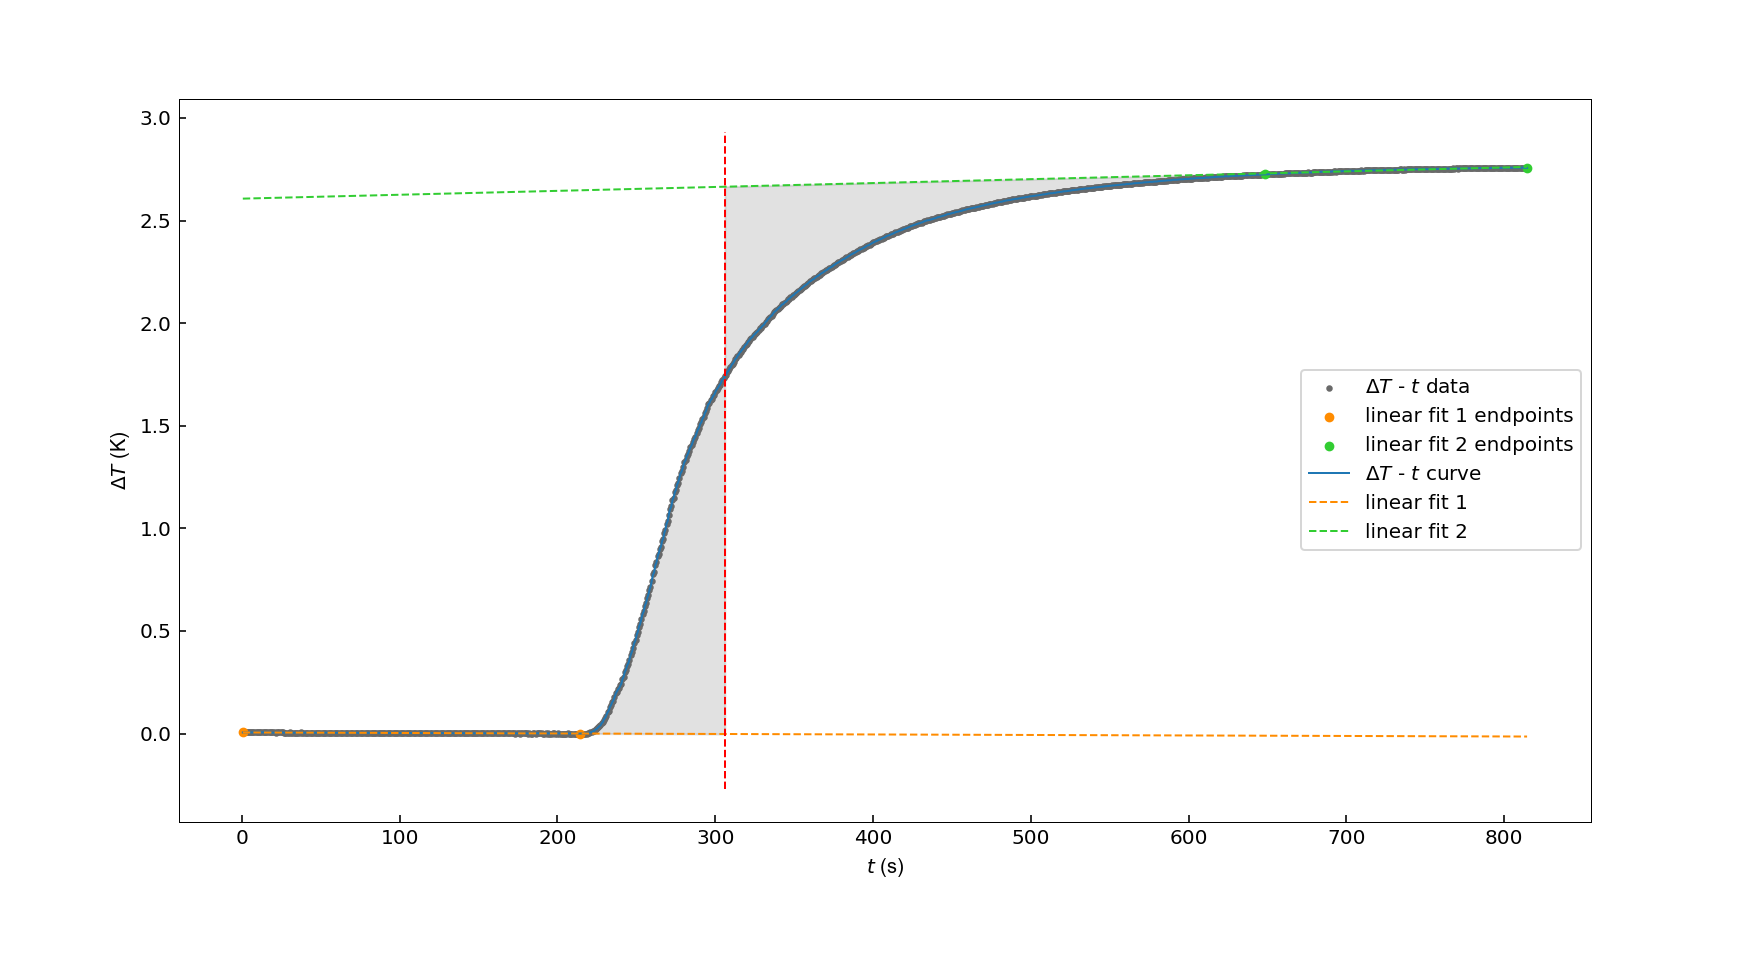
\includegraphics[width = .90\textwidth]{image/r3.png}
    \caption{第三轮实验温差随时间变化图}\label{7}
\end{figure}

使用雷诺校正可以得到燃烧前后的温度 $T_{before} = -0.002\ K,\ T_{after} = 2.665\ K$ ,温差为 $\Delta T = 2.667\ K$。
得到每克样品温升值为:
$$
\Delta T_m = 1.314\ K/g
$$

由上可知,氧弹式量热计常数为 2553.5 J/K ,因此量热计吸热为 6810 J。水的比热容为 4.1852 $\rm J\cdot g^{-1}\cdot K^{-1}$,因此水的吸热为
33452 J。

由公式
\begin{equation*}
    \begin{split}
    Q_V &= - \frac{(W+DC_{H_2O})\Delta T + \sum{q}}{G}  \\
        &=  \frac{ 6810 + 33452 + ( 0.0132 - 0.0102)\times (-3243) +  0.0148 \times (- 16736)}{2.0285} \\
        &= 19721 J/g
    \end{split}
\end{equation*}

可以计算得到奶片的燃烧热为 19721 J/g。由 \ref{114} 的讨论可知,主要的误差来源为水的定容误差与水的量热器常数误差。
$$
\sigma_{Q_V} = \frac{\Delta T}{G}  \times (C_{H_2O} \times \frac{e}{\sqrt{3}} + \sigma_W)  = 2 \times 10^1\ J/g
$$

因此奶片的燃烧热 $Q_V = 1.972 \times 10^4 \pm 2 \times 10^1\ J/g$。由于查询不到伊利奶片的摩尔燃烧热的真实值,因此不能计算与真实值的误差分析。

\subsection[short]{不使用软件的雷诺校正}

使用软件 Origin 对第三轮实验的数据进行雷诺校正,对实验中的两段平台期进行线性拟合,结果为:
$$
\Delta T = (-2.44\times10^{-5} \pm 4\times10^{-7}) t + (0.00506 \pm 5\times10^{-5}) \quad R^2 = 0.926
$$
$$
\Delta T = (1.90\times10^{-4} \pm 3\times10^{-6}) t + (2.607 \pm 0.002) \quad R^2 = 0.954
$$
绘制图像图所示。取第一段平台期最后一个点的纵坐标与第二段平台期第一个点的纵坐标,
取其平均值并作出垂线与曲线图以及两条拟合直线。可以测得经
雷诺校正后的温差为得到温差为 2.575 K。
\begin{figure}[htbp]
    \centering
    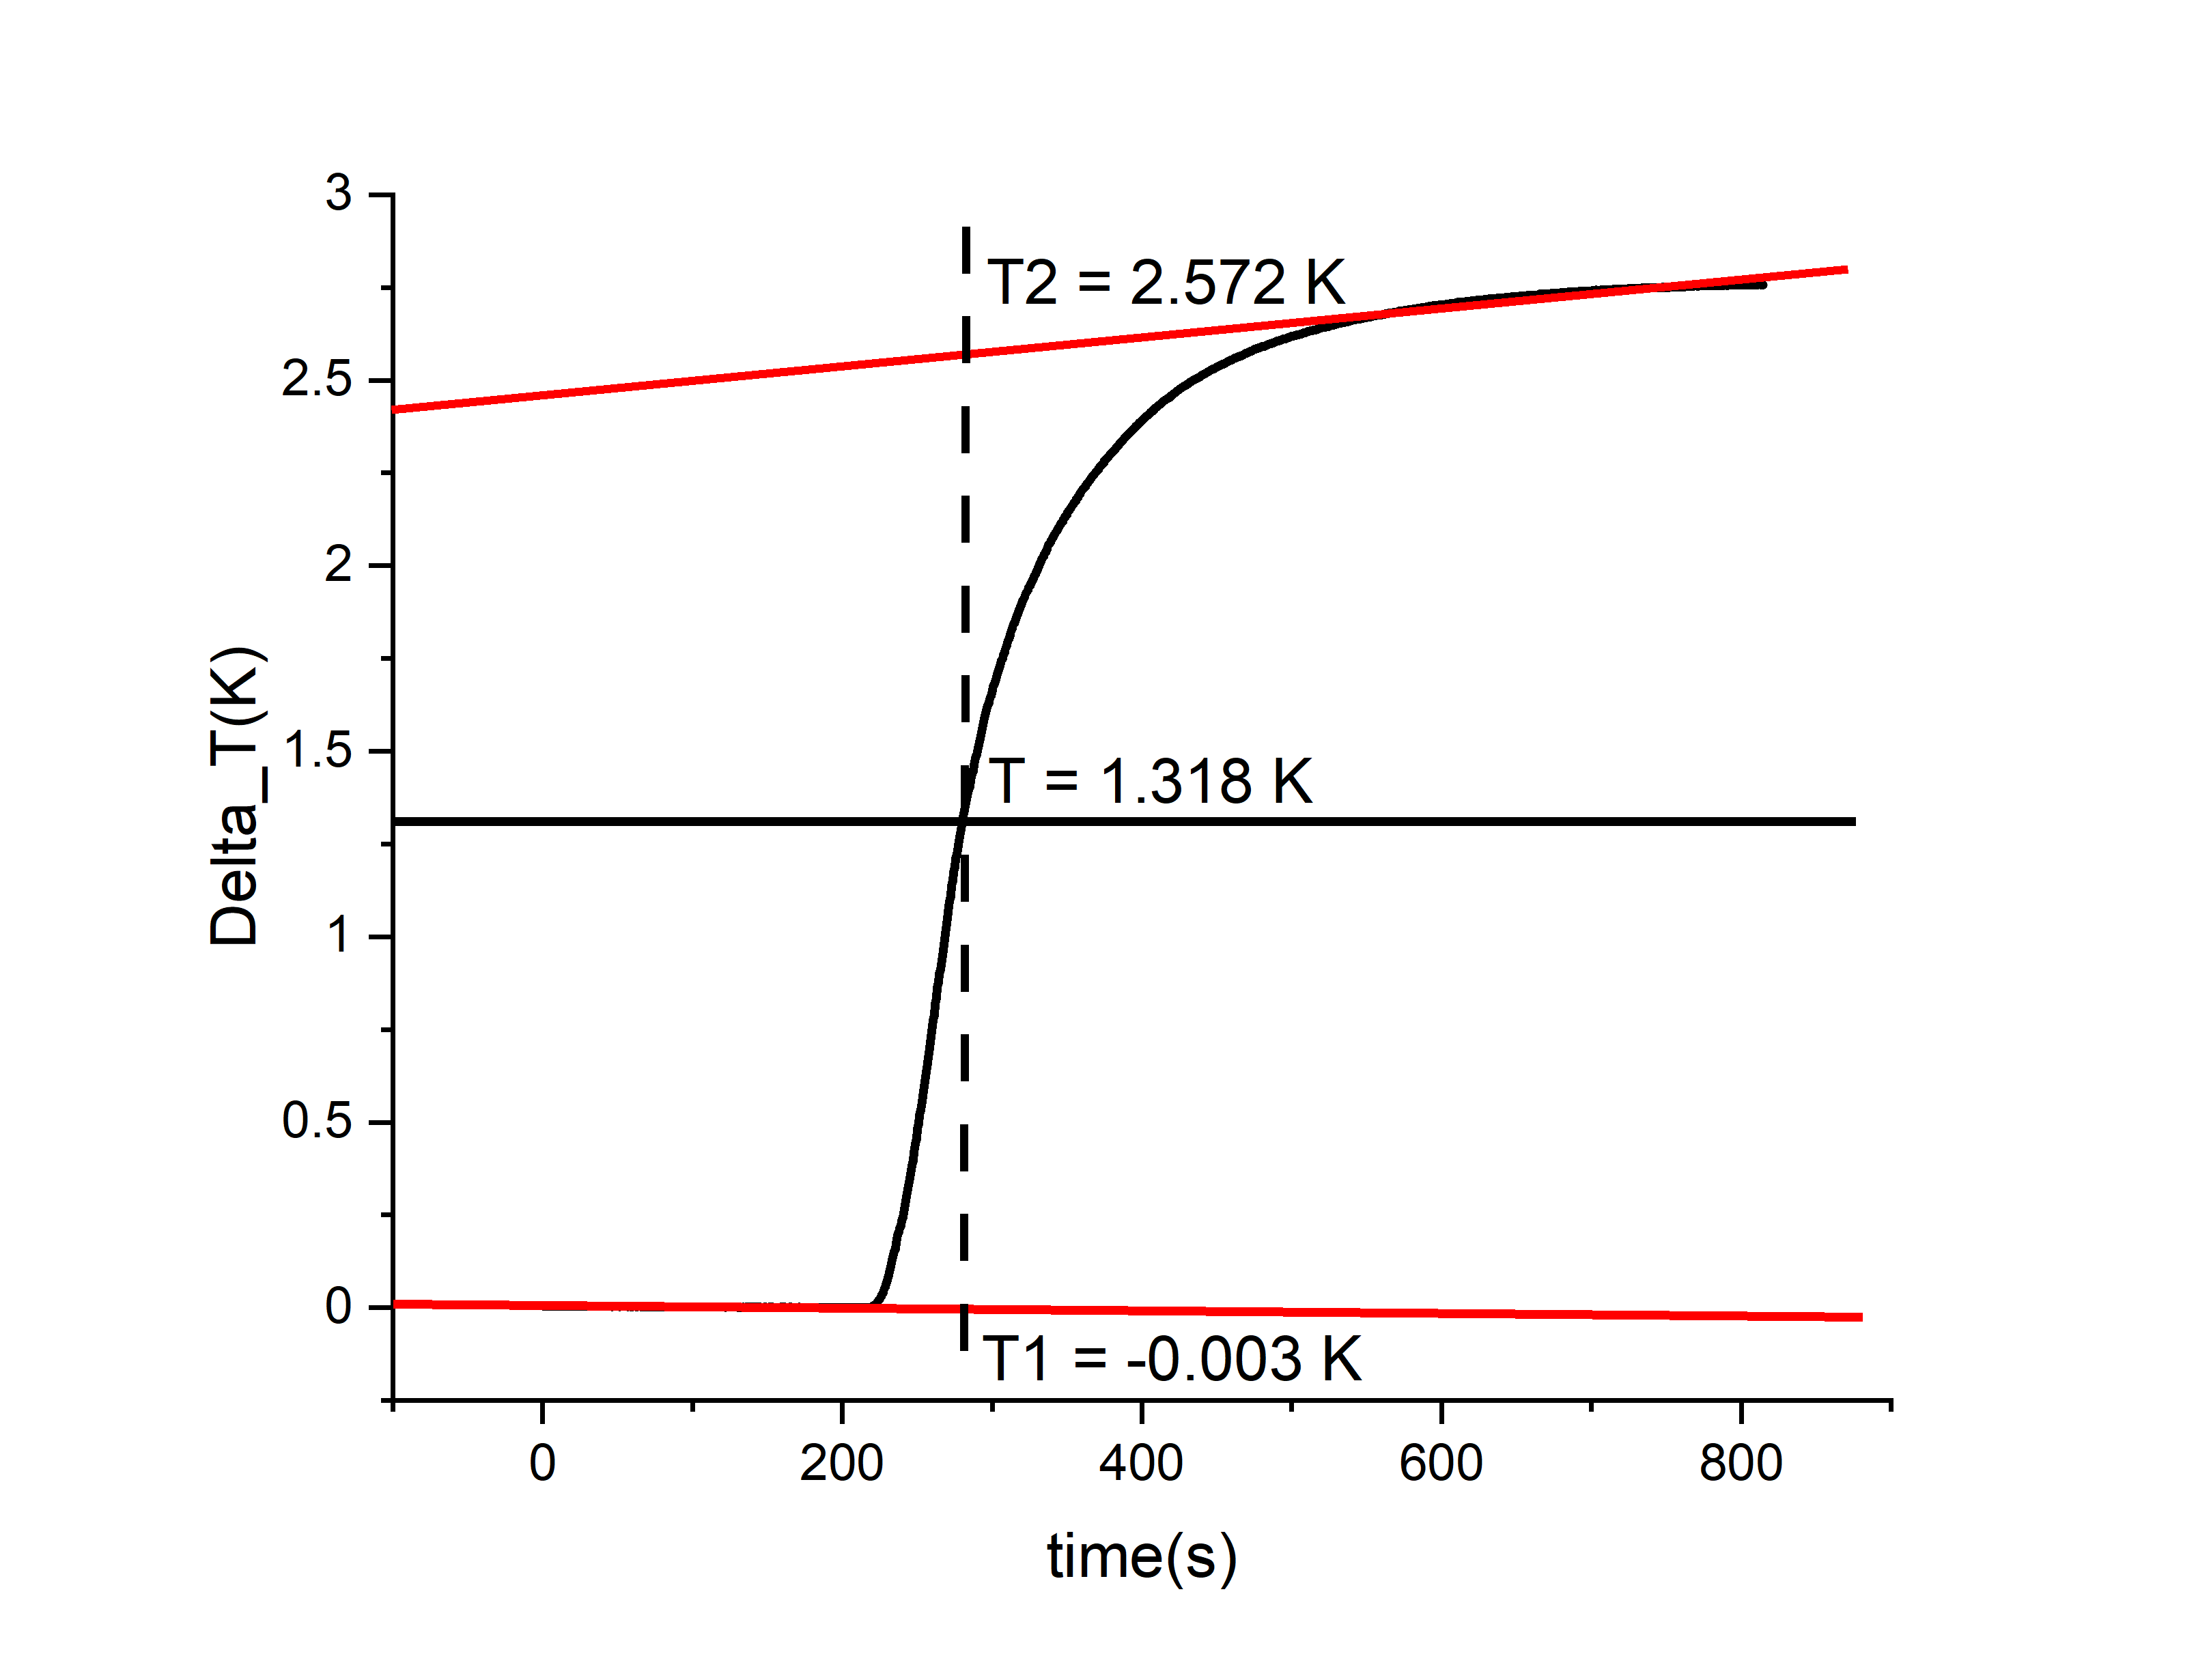
\includegraphics[width = .70\textwidth]{image/Graph1.png}
    \caption{第三轮实验不使用软件的雷诺校正}\label{8}
\end{figure}


\section{实验结果与讨论}

\subsection{结论}

本实验有三轮实验,分别测定蔗糖、苯甲酸以及奶片的燃烧热
。通过已知的苯甲酸燃烧热测定了氧弹的水当量,使用雷诺校正法修正了
燃烧过程中环境热交换,最后测定奶片的恒容燃烧热。

实验得到,得到每克蔗糖温升值为 $\Delta T_m = 0.098\ K/g$ ,
量热计常数为 $ W = 2553 \pm 9 J/K$,奶片的燃烧热 $Q_V = 1.972 \times 10^4 \pm 2 \times 10^1\ J/g$
,实验中误差的主要来源是容量瓶的定容误差。

\nocite{*}
\bibliography{reference}
\end{document}
